\chapter{Componentes de uma Criptomoeda}
\label{ch:bitcoin-tech}

\section{Considerações Iniciais}

Este capítulo apresenta um resumo dos componentes básicos de uma criptomoeda como o Bitcoin para servir de introdução ao capítulo seguinte.

\section{Endereços}

As criptomoedas baseiam-se no esquema de criptografia de chaves públicas e privadas, sendo o algoritmo ECDSA implementado no Bitcoin. Cada usuário possui um conjunto de chaves públicas gerados a partir de chaves privadas. As chaves públicas são então usadas para gerar um \textit{hash} de 160 bits que depois é codificado com Base58Check em uma \textit{string} alfa-numérica começando com o dígito 1 ou 3 (Figura~\ref{fig:endereco}). Essa \textit{string} final é chamada de endereço\footnote{\cite[p. 71]{bib:bitcoinbook}.}. Usuários podem gerar novos endereços indefinidamente e, como prática comum para preservar a pseudoanonimidade, usa-se um endereço novo a cada vez que se recebe uma transação.

\begin{figure}[h!]
	\centering
	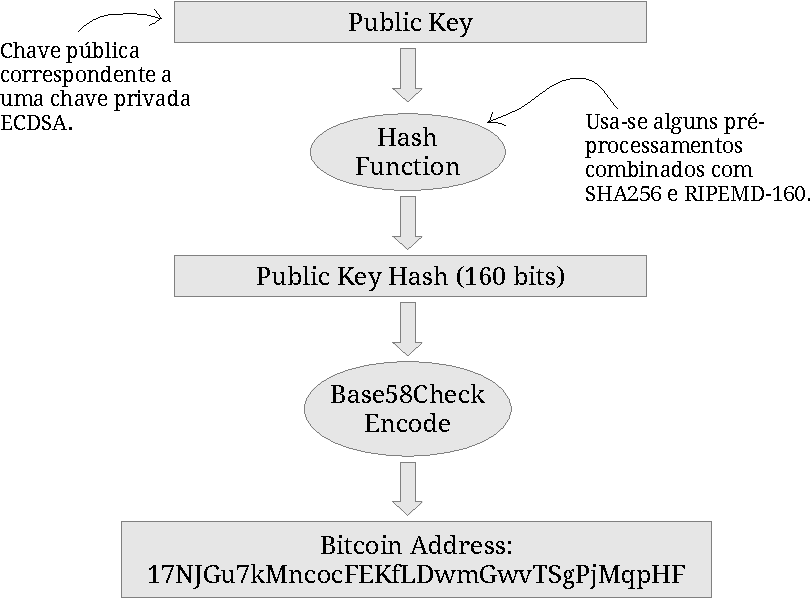
\includegraphics[scale=0.85]{./images/endereco.pdf}
	\caption{Ilustração simplificada do processo de criação de um endereço. \label{fig:endereco}}
\end{figure}

\section{Transações}

As transações possuem endereços de entrada e de saída e são feitas diretamente de endereço para endereço. Como ilustra a Figura~\ref{fig:transacao}, mais do que um endereço pode ser usado na entrada para compor o valor que se deseja transferir e mais do que um endereço pode ser informado na saída. O valor total de saída deve ser menor ou igual ao valor total de entrada --- caso seja menor, a diferença é dada como \textit{taxa de transação} para o minerador que incorporar a transação em seu bloco, como será explicado na Seção~\ref{sec:mineracao}. Para autenticar uma transação, ela deve ser assinada digitalmente pelos endereços de entrada com suas chaves privadas.

\begin{figure}[h!]
	\centering
	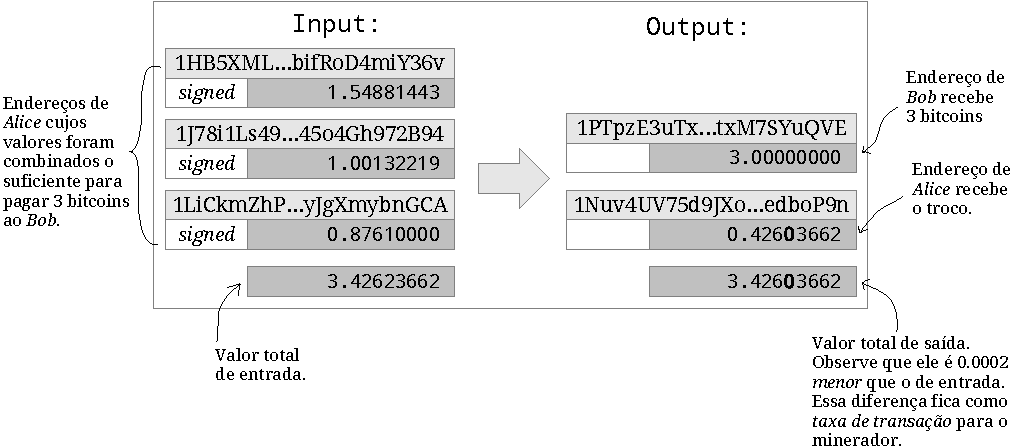
\includegraphics[scale=1]{./images/transacao.pdf}
	\caption{Ilustração simplificada de uma transação em que Alice transfere 3 bitcoins para Bob. \label{fig:transacao}}
\end{figure}

Os usuários dispõem de um certo nível de privacidade devido ao uso de endereços, porém eles não são anônimos na rede. Analisando as transações na blockchain e associando informações sobre alguns endereços já pré-identificados, pode-se inferir sobre as identidades reais de outros endereços \cite{bib:anonimidade}. Por esse motivo, usa-se o termo \textit{pseudoanônimo} para se referir ao nível de privacidade do Bitcoin. Existem técnicas para melhorar a anonimidade, como \textit{mixing services}, mas ainda não o suficiente para garantir que os usuários sejam anônimos.

\section{Carteiras}

As carteiras, \textit{wallets}, são aplicativos de computador/smartphone/Web capazes de guardar chaves privadas e gerenciar um conjunto de endereços, acompanhando o valor total deles e realizando operações: criar, assinar e enviar transações. Geralmente, fazem uso de \textit{QR code} para ler mais facilmente os endereços. A Figura~\ref{fig:carteira} mostra um exemplo de carteira para smartphone com sistema operacional Android. Uma carteira não necessariamente precisa ser um nó completo na rede, ela pode operar de maneira mais leve, consultando apenas blocos de seu interesse para verificar suas transações. Existem atualmente três tipos de tecnologias de carteira:
\begin{itemize}
	\item \textbf{Não-determinística (aleatória)}: a primeira versão de carteira que consiste em um conjunto de chaves privadas aleatórias. Gera-se um conjunto de $n$ chaves privadas aleatórias e posteriormente gera-se mais chaves conforme necessário. O backup desse tipo de carteira é trabalhoso, pois precisa ser mais frequente uma vez que é necessário manter uma cópia de cada nova chave privada.

	\item \textbf{Determinística (usa uma semente)}: contém chaves privadas que são geradas a partir de uma única semente. Somente o backup da semente já é suficiente para recuperar todas as chaves derivadas.
	
	\item \textbf{Determinística Hierárquica + Mnemônica}: usa uma técnica mais sofisticada e rápida\footnote{BIP 0032. Disponível em: \url{https://github.com/bitcoin/bips/blob/master/bip-0032.mediawiki}. Acesso em: 12 abr. 2016.} para derivação de chaves privadas a partir de uma semente. A semente é codificada em um formato literal por um sequência de 12 ou 24 palavras.
\end{itemize}

\begin{figure}[h!]
	\centering
	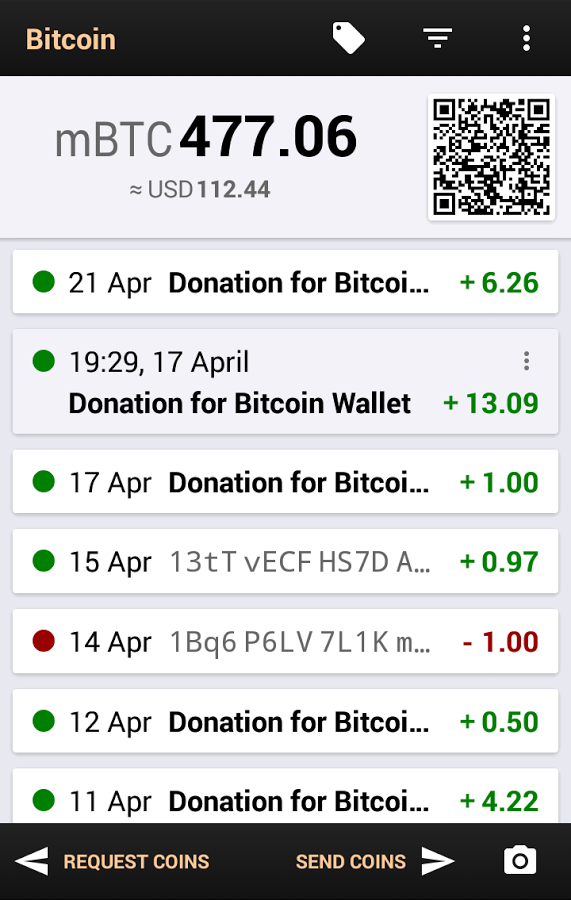
\includegraphics[scale=0.32]{./images/carteira.png}
	\caption[Exemplo de uma aplicativo de carteira: Bitcoin Wallet para Android.]{Exemplo de uma aplicativo de carteira: Bitcoin Wallet para Android\protect\footnotemark. \label{fig:carteira}}
\end{figure}
\footnotetext{Disponível em: \url{https://play.google.com/store/apps/details?id=de.schildbach.wallet}. Acesso em: 13 abr. 2016.}

\textbf	{Importante}: carteiras não guardam moedas; carteiras guardam chaves privadas e seus respectivos endereços. Dizer que alguém possui 1 bitcoin significa dizer que: ele possui as chaves privadas que geram as chaves públicas cujos endereços estão registrados na blockchain e a soma dos valores atribuídos a esses endereços é de 1 bitcoin. Ou, de maneira simplificada, dizer que alguém possui 1 bitcoin significa dizer que: a \textbf{rede consente} que o detentor de tais endereços possui 1 bitcoin.

\section{Blockchain}

Blockchain é um banco de dados público, distribuído pela Internet entre os mineradores. Nele são registradas todas as transações realizadas com a criptomoeda. O significado do nome vem de sua implementação: estruturas de dados em que um bloco de dados ``aponta'' (possui um ponteiro) para o bloco anterior, ``seu bloco pai'', formando uma cadeia de blocos (Figura~\ref{fig:blockchain}). Esse ponteiro é implementado utilizando o \textit{hash} do bloco anterior, mantendo assim a integridade dos dados na cadeia, pois qualquer modificação em dados anteriores mudará o valor do \textit{hash} do ponteiro. Cada bloco contém um conjunto de transações que é acessível por meio de uma árvore de dados que também implementa ponteiros \textit{hash} (Merkle Tree).

O processo de mineração incrementa essa cadeia adicionando um novo bloco no final (\textit{append-only}). Logo, todas as transações contidas nesse bloco são salvas e quanto mais mineradores consentirem que determinado bloco faz parte da blockchain, mais efetivamente as transações desse bloco estão confirmadas.

\section{Mineração}
\label{sec:mineracao}

Mineração é o processo pelo qual novas unidades de moeda são inseridas na rede. A mineração também é responsável por realizar as transações e pela segurança da rede contra fraudes, ataques e gastos duplos.

Os \textbf{mineradores} são nós na rede que guardam uma cópia dos registros das transações (blockchain) e executam a atividade de mineração. Eles competem para ``encontrar o próximo bloco'' --- jargão para o processo de \textit{Proof-of-Work}: um trabalho difícil de ser feito, porém fácil de ser verificado. No Bitcoin, ele consiste em encontrar um \textit{nonce} tal que o \textit{hash} do cabeçalho do bloco seja inferior a um determinado coeficiente de dificuldade (\textit{target}). Essa dificuldade é por definição ajustada a cada 2016 blocos de modo que se mantenha a taxa esperada de 1 bloco a cada 10 minutos\footnote{Mais informações em: \url{https://en.bitcoin.it/wiki/Difficulty}. Acesso em: 12 abr. 2016.}.

Dessa forma, uma vez que um minerador encontra o \textit{nonce} que satisfaz o \textit{hash} do bloco em que está trabalhando, ele faz broadcasting desse novo bloco na rede. Os demais mineradores verificam a legitimidade do bloco e então o aceitam, incorporando-o em sua cópia da blockchain. Esse ato de aceitação é chamado de \textbf{confirmação} e normalmente usa-se a heurística de pelo menos 6 confirmações para considerar que um bloco efetivamente faz parte da blockchain. O protocolo dos mineradores é o de sempre seguir com a cadeia mais longa.

Como a rede é descentralizada e os nós podem entrar e sair de maneira independente, não é possível contabilizar a quantidade de nós em operação para dar-lhes uma recompensa pelo seu trabalho prestado. Assim, o \textit{Proof-of-Work} promove uma distribuição justa de recompensas, pois a probabilidade de um nó ``encontrar o próximo bloco'' é proporcional ao seu poder computacional dentro da rede. Atualmente, para cada novo bloco inserido na blockchain, o minerador ganha 25 unidades de bitcoin (cerca de R\$ 41.125,00) e por definição esse valor diminui pela metade a cada 210\,000 blocos (cerca de 4 anos). Essa recompensa representa a \textbf{emissão} de novas unidades de moeda e é realizada por meio de uma transação especial, chamada \textit{coinbase transaction}, criada pelo próprio minerador e atribuída a um endereço de sua escolha.

\begin{figure}[h!]
	\centering
	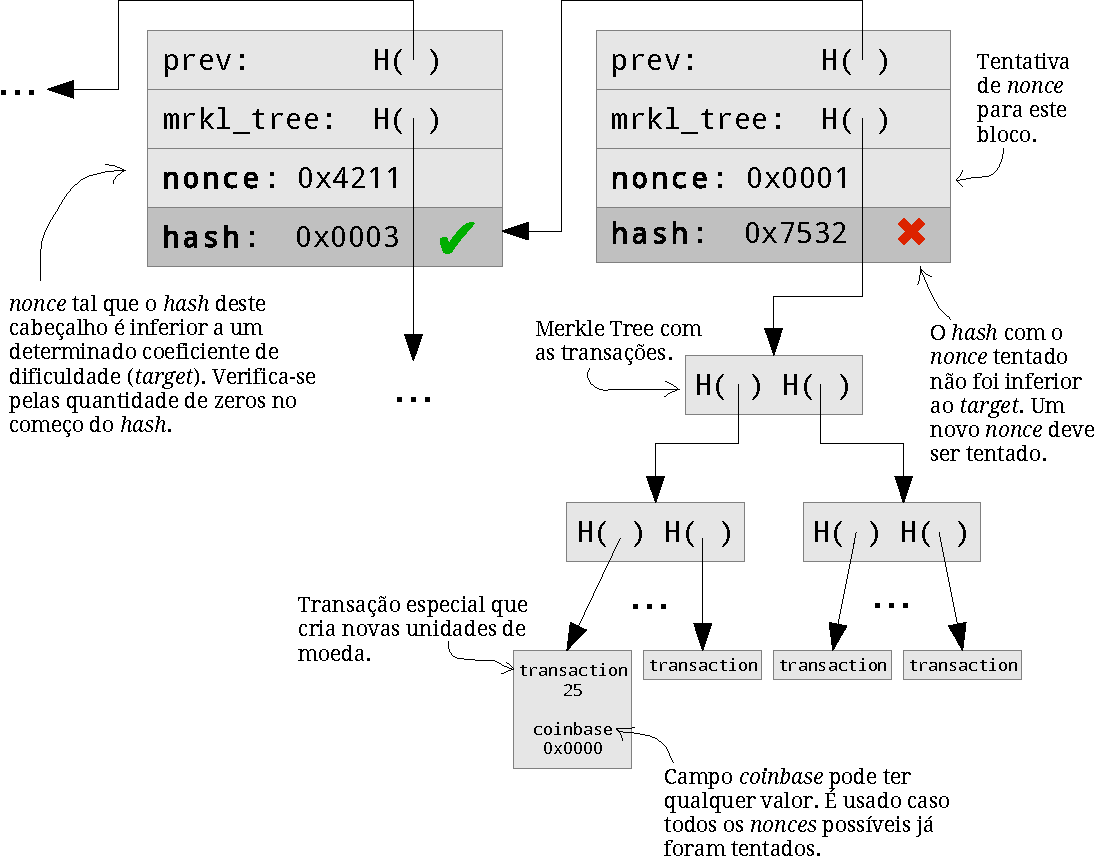
\includegraphics[scale=0.85]{./images/blockchain.pdf}
	\caption[Ilustração simplificada da estrutura de dados na blockchain.]{Ilustração simplificada da estrutura de dados na blockchain\protect\footnotemark. \label{fig:blockchain}}
\end{figure}
\footnotetext{Adaptação de \cite[Fig. 5.1]{bib:princeton-book}.}

O \textit{Proof-of-Work} também fortalece a segurança da rede, pois para fraudar um bloco é sempre necessário refazer o trabalho de encontrar o \textit{nonce} e, conforme a blockchain cresce e se espalha pela rede confirmando o consenso, mais difícil a fraude. Dessa maneira, pode-se dizer que o bitcoin é o primeiro produto digital e escasso ao mesmo tempo, pois seu protocolo implica que somente uma cópia de cada transação seja registrada na blockchain.

Outra forma de recompensa é por meio das \textbf{taxas de transação} cobradas pelos mineradores para incluir uma transação em seu bloco. Ela é usada para definir prioridades entre as transações e evitar \textit{spam}. O autor de uma transação, ao informar o valor total de entrada maior que o valor total de saída, está dando a diferença como taxa para o minerador que incluir aquela transação em seu bloco. O autor da transação pode escolher pagar uma taxa de valor zero, porém corre o risco de ter sua transação ignorada pelos mineradores. Historicamente, essa taxa não era requerida, mas hoje quase todos mineradores esperam receber taxas e no futuro, quando a recompensa por encontrar blocos for reduzida a zero, as taxas de transação serão o principal meio de recompensa para os mineradores.

Existe uma gama de tópicos que envolvem a mineração, entre eles, mineração em \textit{pools}, \textit{51\% attack}, DoS, consenso distribuído, teoria dos jogos etc, mas resumidamente pode-se dizer que os mineradores executam quatro funções: $i)$ armazenam e propagam a blockchain, $ii)$ validam novas transações, $iii)$ emitem novas unidades da criptomoeda e $iv)$ votam em um consenso com seu poder computacional.

Vista a possibilidade de descentralizar a moeda, os entusiastas já pensam adiante: ``Por que não descentralizamos tudo?''. A blockchain e o processo de mineração tornam-se os principais objetos de estudo para alcançar a descentralização em outros serviços na sociedade, como contratos, licenças, declarações de propriedade etc.

\section{Bootstrapping}

Tecnicamente criar uma nova criptomoeda é uma tarefa facilitada devido aos projetos de criptomoedas serem de código-fonte aberto. Porém, existe um difícil caminho para conseguir que ela adquira valor e seja comumente aceita como meio de troca. Esse processo, chamado de \textit{bootstrapping}, envolve conquistar mineradores, \textit{stakeholders}, desenvolvedores e atingir uma liquidez satisfatória. Durante essa fase, enquanto não se consegue uma quantidade razoável de mineradores interessados em participar do projeto, a nova criptomoeda é sensível a ataques e portanto insegura. Logo, essa é uma etapa difícil e técnicas são necessárias para se suceder.

Para a criptomoeda obter valor, é necessário adquirir qualidades que incentivem as pessoas a valorizá-la. Uma comunidade de desenvolvedores fortalece a moeda, pois cria-se a confiança de que ela está sendo pesquisada e aprimorada (correção de bugs, implementação de novas funcionalidades, melhorias na segurança e escalabilidade etc). Assim como pessoas interessadas em comprar/vender a moeda por outras moedas, ou melhor, negociar um produto/ serviço diretamente na nova moeda, criam a confiança de que ela pode ser usada como meio de troca.

\section{Considerações Finais}

A implementação dos componentes aqui apresentados é composta de técnicas sofisticadas de engenharia de software e criptografia. Importante ressaltar que o Bitcoin é um software crítico e que tem recebido contribuições de profissionais altamente capacitados da área de computação.